\setlength{\columnsep}{3pt}
\begin{flushleft}

Type of IP address depends on:
\begin{itemize}
	\item \textbf{Location}: There are 2 types of IP address:
	\begin{figure}[h!]
		\centering
		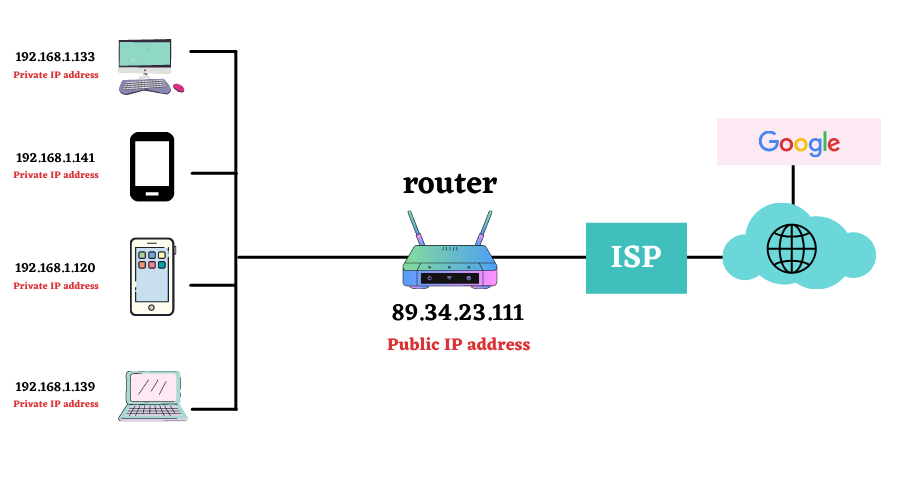
\includegraphics[scale=0.4]{content/chapter14/images/public_private.png}
		\caption{Public \& Private IP}
		\label{fig:public_private_ip}
	\end{figure}
	
	\begin{itemize}
		\item \textbf{Public IP address}: Used \textbf{outside of a network}.
		\item \textbf{Private IP address}: Used \textbf{inside a network}.
	\end{itemize}
	\bigskip
	\bigskip
	\item \textbf{Permanancy}: There are 2 types of IP address:
	\begin{figure}[h!]
		\centering
		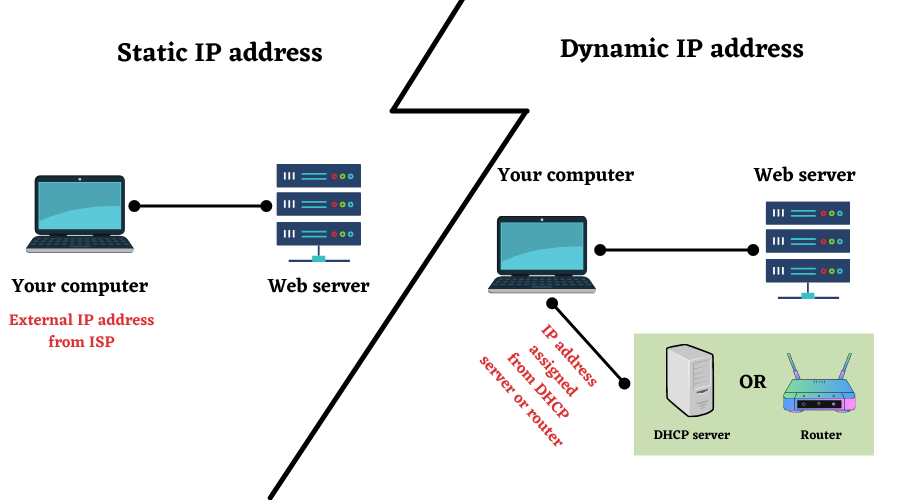
\includegraphics[scale=0.4]{content/chapter14/images/static_dynamic.png}
		\caption{Static \& Dynamic IP}
		\label{fig:s_d_ip}
	\end{figure}
	\begin{itemize}
		\item \textbf{Static IP address}: \textbf{Won't change and created manually}. Provided by ISP provider for external usage. 
		\item \textbf{Dynamic IP address}: \textbf{Can change anytime} and assigned by a \textbf{Dynamic Host Configuration Protocol (DHCP)} server or router.
	\end{itemize}
\end{itemize}

	

	

	
	

	
	
	
\end{flushleft}
\newpage


